\documentclass{article}

\usepackage{blindtext}
\usepackage{graphicx}
\usepackage{subcaption}
\usepackage{url}
\usepackage{fixltx2e}
%\usepackage{subcaptions}

\pagenumbering{gobble}

\begin{document}

\title{carica e scarica di un condensatore}
\author{Ionut Cicio 3Binf.}
\date{02/02/2020}

\maketitle

\section*{Obiettivo}
Dimostrare e spiegare il funzionamento di carica e di scarica di un condensatore,
simulando i due circuiti su qucs, ed elaborando i grafici risultanti dalla simulazione.

\section*{Strumenti}
qucs versione 0.0.19 (\url{http://qucs.sourceforge.net/})

\section*{Spiegazione teorica}

\subsection*{definizione}
Il condensatore e un componente elettronico che ha la capacita' di immagazinare energia sotto forma di campo elettrostatico. \\
Tale energia, nel caso di un condensatore ideale, viene conservata all'infinito (nel caso reale, essendo che tutto e' fatto di materiale, tutto ha una resistenza, per cui, anche se dopo molto, il condensatore si scarica)

\subsection*{composizione}
Il condensatore e' composto da due conduttori detti armature, o piatti, separati da un materiale isolante detto dielettrico

\subsection*{formule e grafici}
C=$\epsilon$\textsubscript{0}$\epsilon$\textsubscript{r}$\frac{S}{d}$

%\caption{caption}
%\label{fig:label}

\newpage

\section*{circuito di carica}

\begin{figure}[h!]
  \centering
  \begin{subfigure}[b]{0.3\linewidth}
    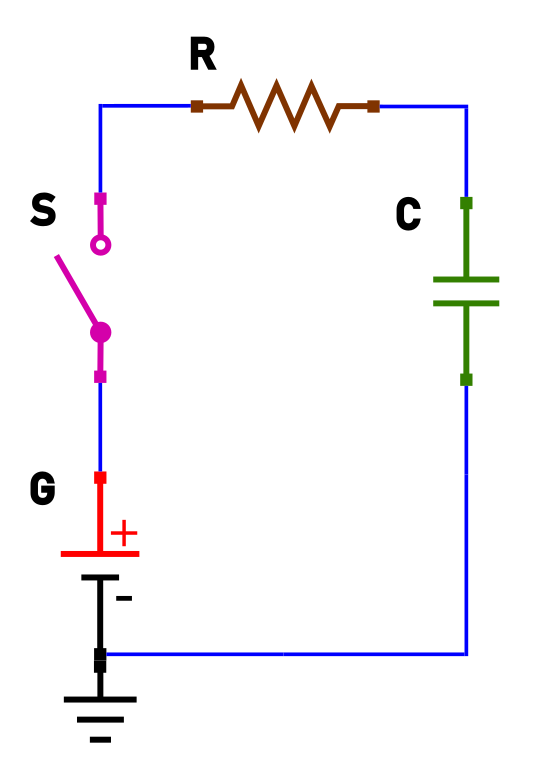
\includegraphics[width=\linewidth]{data/carica-open.png}
  \end{subfigure}
  \begin{subfigure}[b]{0.3\linewidth}
    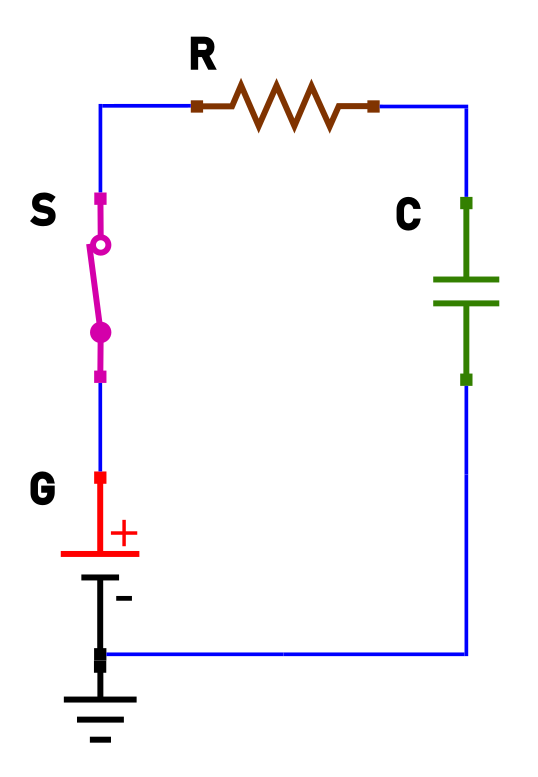
\includegraphics[width=\linewidth]{data/carica-closed.png}
  \end{subfigure}
  \begin{subfigure}[b]{0.347\linewidth}
    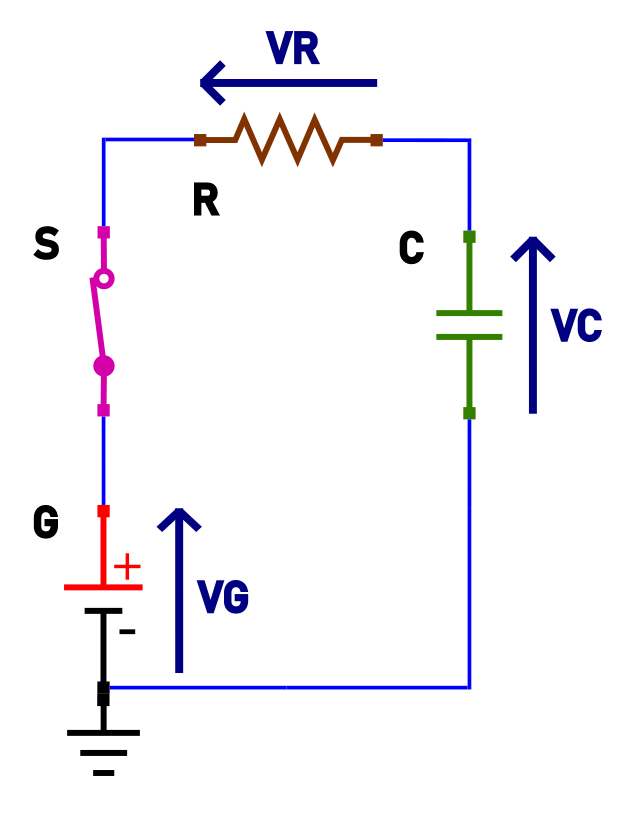
\includegraphics[width=\linewidth]{data/carica-tensioni.png}
  \end{subfigure}
\end{figure}

\subsection*{grafici carica}
\begin{figure}[h!]
  \centering
  \begin{subfigure}[b]{0.3\linewidth}
    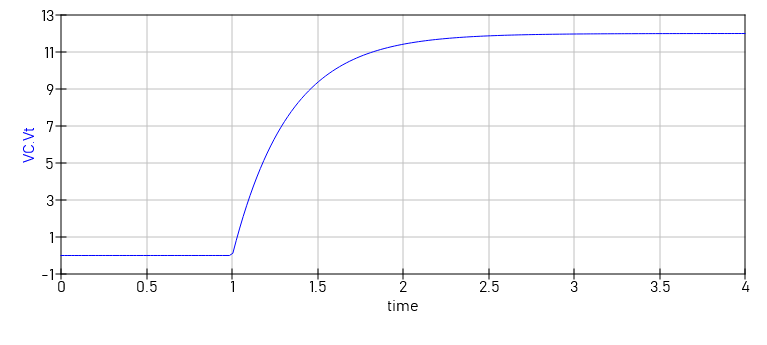
\includegraphics[width=\linewidth]{data/carica-VC.png}
  \end{subfigure}
  \begin{subfigure}[b]{0.3\linewidth}
    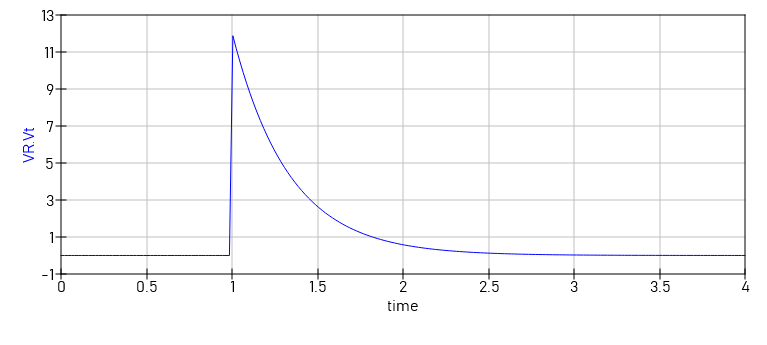
\includegraphics[width=\linewidth]{data/carica-VR.png}
  \end{subfigure}
  \begin{subfigure}[b]{0.3\linewidth}
    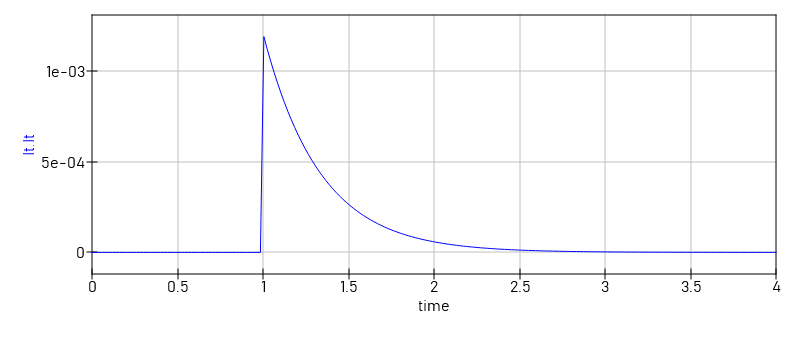
\includegraphics[width=\linewidth]{data/carica-IT.png}
  \end{subfigure}
\end{figure}


\newpage
\section*{circuito di sarica}

\begin{figure}[h!]
  \centering
  \begin{subfigure}[b]{0.3\linewidth}
    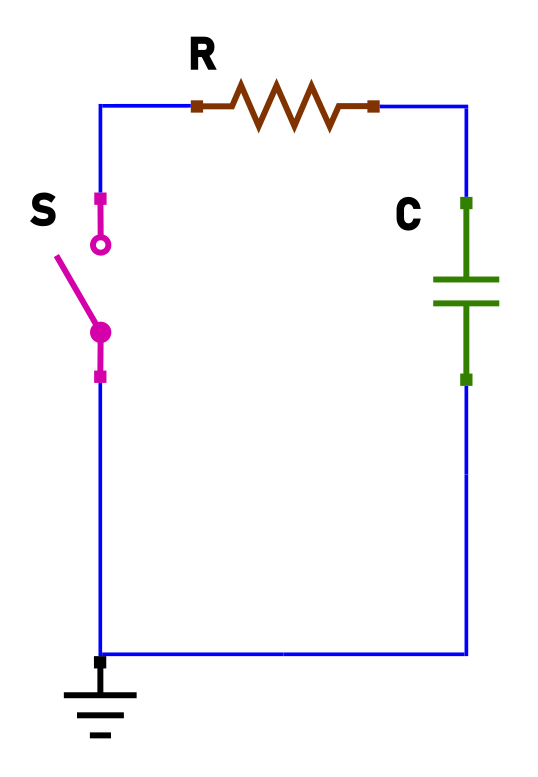
\includegraphics[width=\linewidth]{data/scarica-open.png}
  \end{subfigure}
  \begin{subfigure}[b]{0.3\linewidth}
    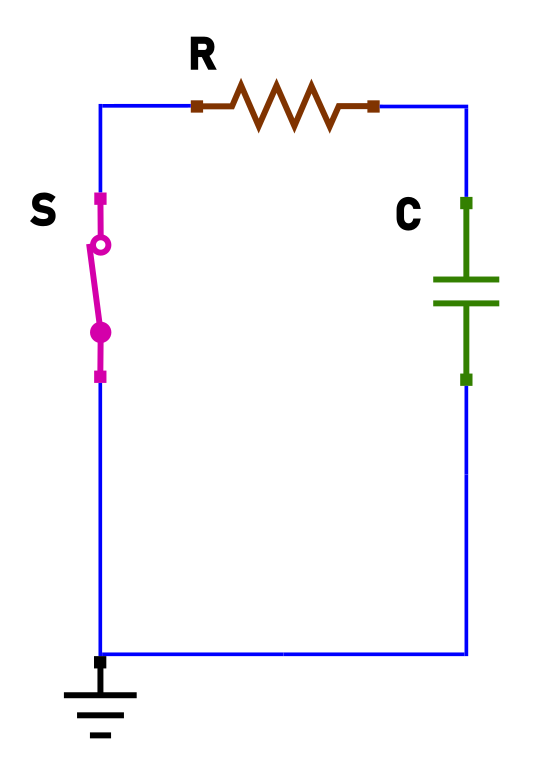
\includegraphics[width=\linewidth]{data/scarica-closed.png}
  \end{subfigure}
  \begin{subfigure}[b]{0.347\linewidth}
    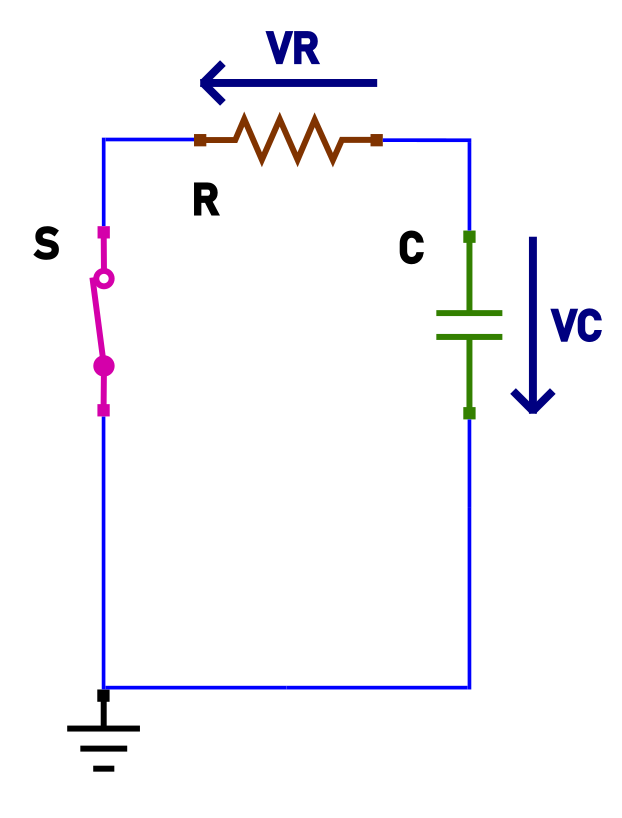
\includegraphics[width=\linewidth]{data/scarica-tensioni.png}
  \end{subfigure}
\end{figure}

\subsection*{grafici scarica}

\begin{figure}[h!]
  \centering
  \begin{subfigure}[b]{0.3\linewidth}
    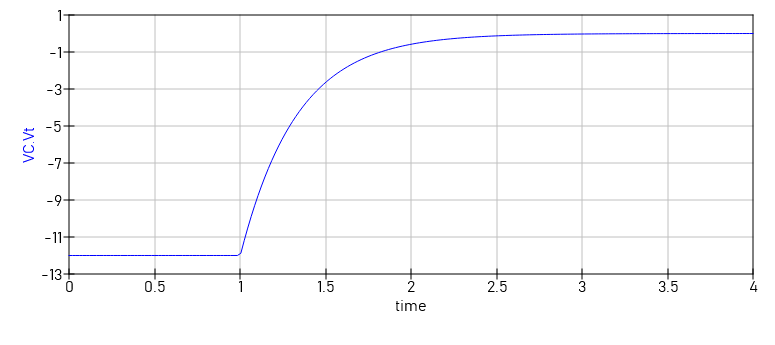
\includegraphics[width=\linewidth]{data/scarica-VC.png}
  \end{subfigure}
  \begin{subfigure}[b]{0.3\linewidth}
    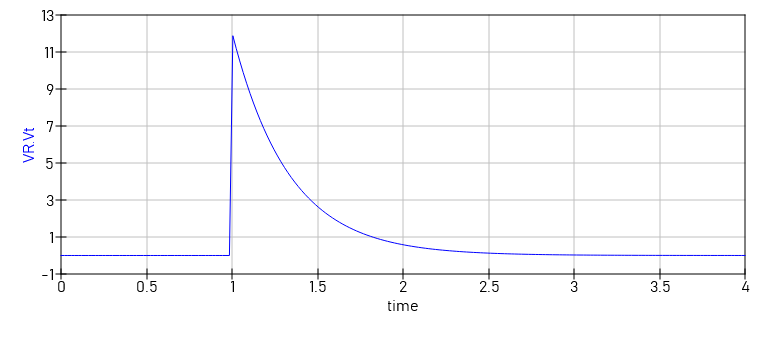
\includegraphics[width=\linewidth]{data/scarica-VR.png}
  \end{subfigure}
  \begin{subfigure}[b]{0.3\linewidth}
    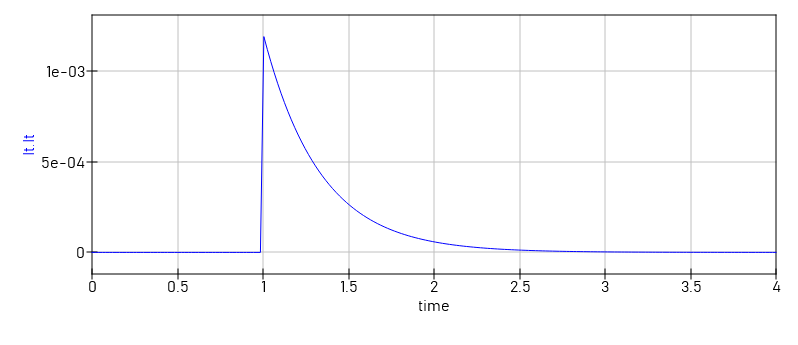
\includegraphics[width=\linewidth]{data/scarica-IT.png}
  \end{subfigure}
\end{figure}

\newpage

\section*{simulazione con qucs}

\subsection*{carica}

\begin{figure}[!h]
  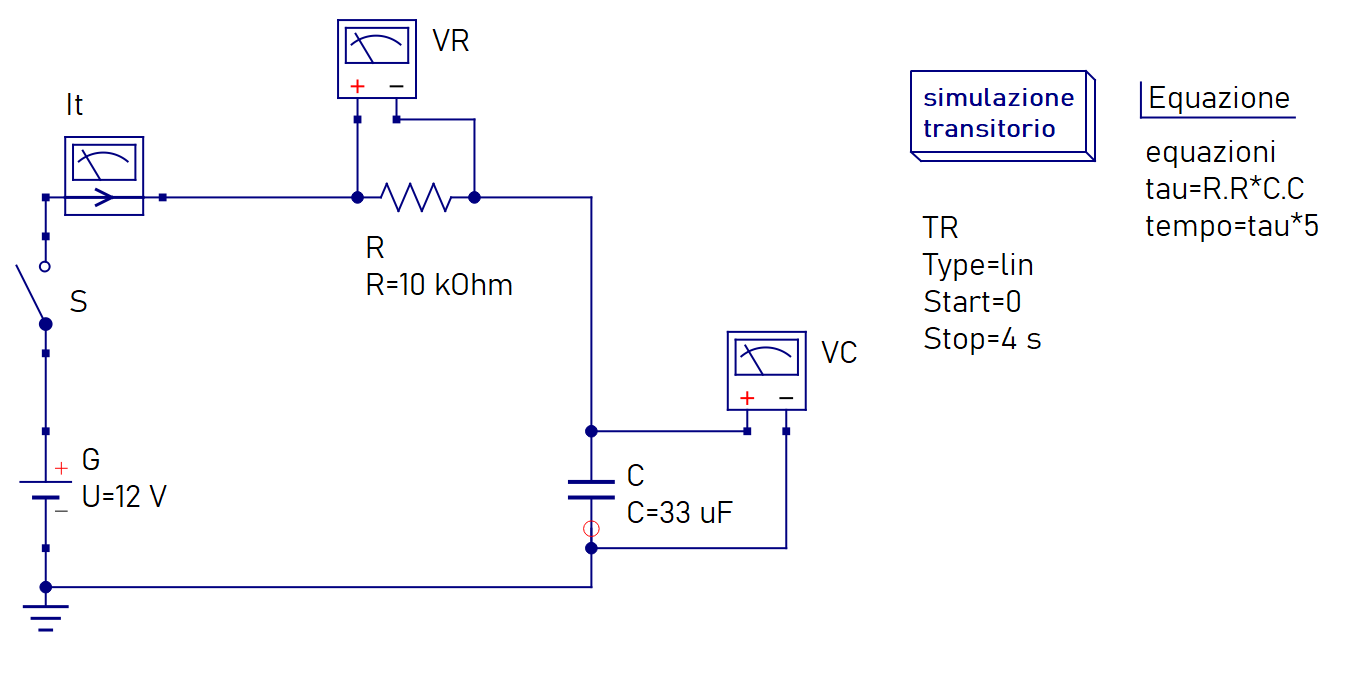
\includegraphics[width=\linewidth]{data/carica-simulazione-qucs.png}
\end{figure}

\subsection*{scarica}

\begin{figure}[!h]
  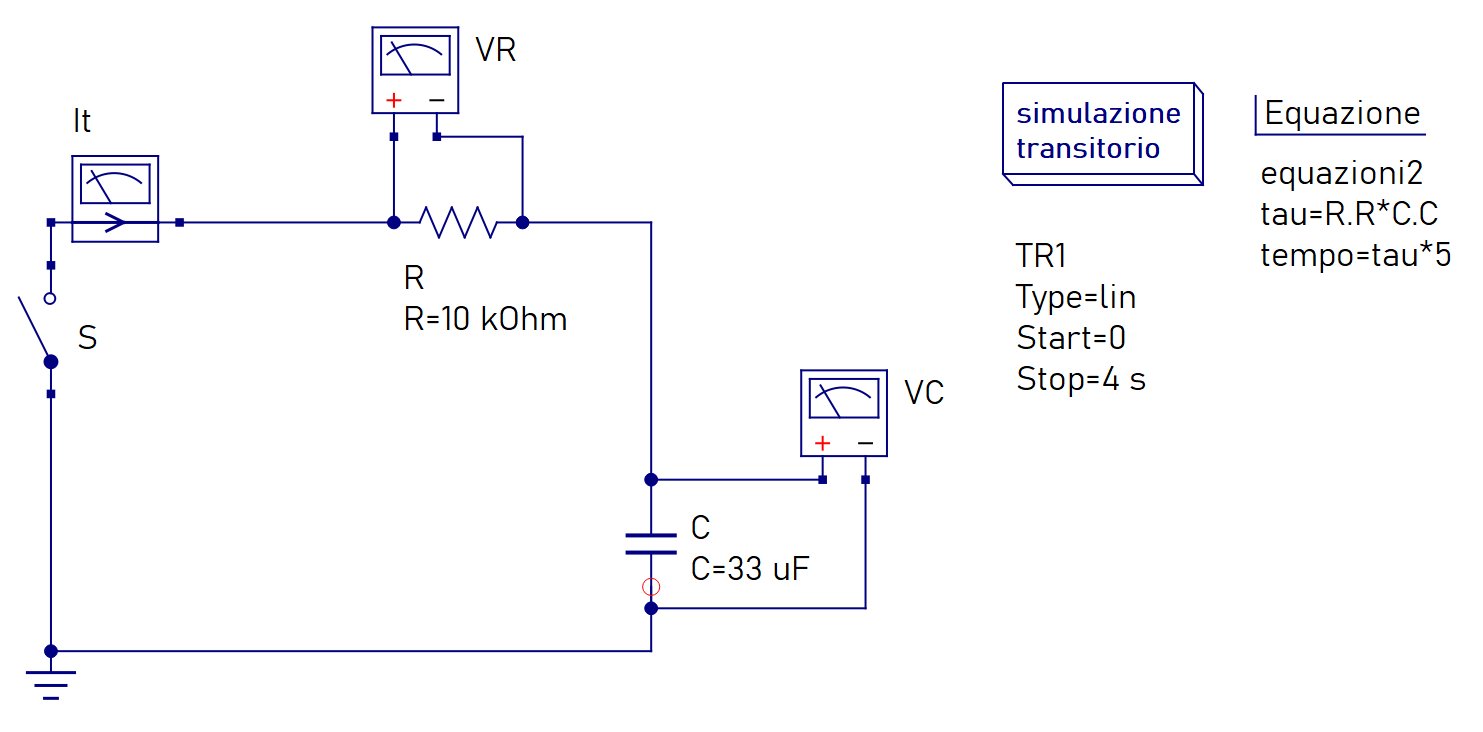
\includegraphics[width=\linewidth]{data/scarica-simulazione-qucs.png}
\end{figure}

\newpage

\section*{conclusioni e osservazioni}
\blindtext[1]


\end{document}